\section{Methods} \label{sec:methods}

This section will introduce the strategy of our hereditary stratigraph approach to decentralized phylogenetic tracking, define the vocabulary we developed to describe aspects of this approach, overview configuration options of the approach, perform mathematical exposition of the properties of the approach under particular configurations, and then recap digital experiments that demonstrate this approach in an applied setting.

\subsection{Hereditary Strata and the Hereditary Stratigraphic Column}

\begin{figure}
    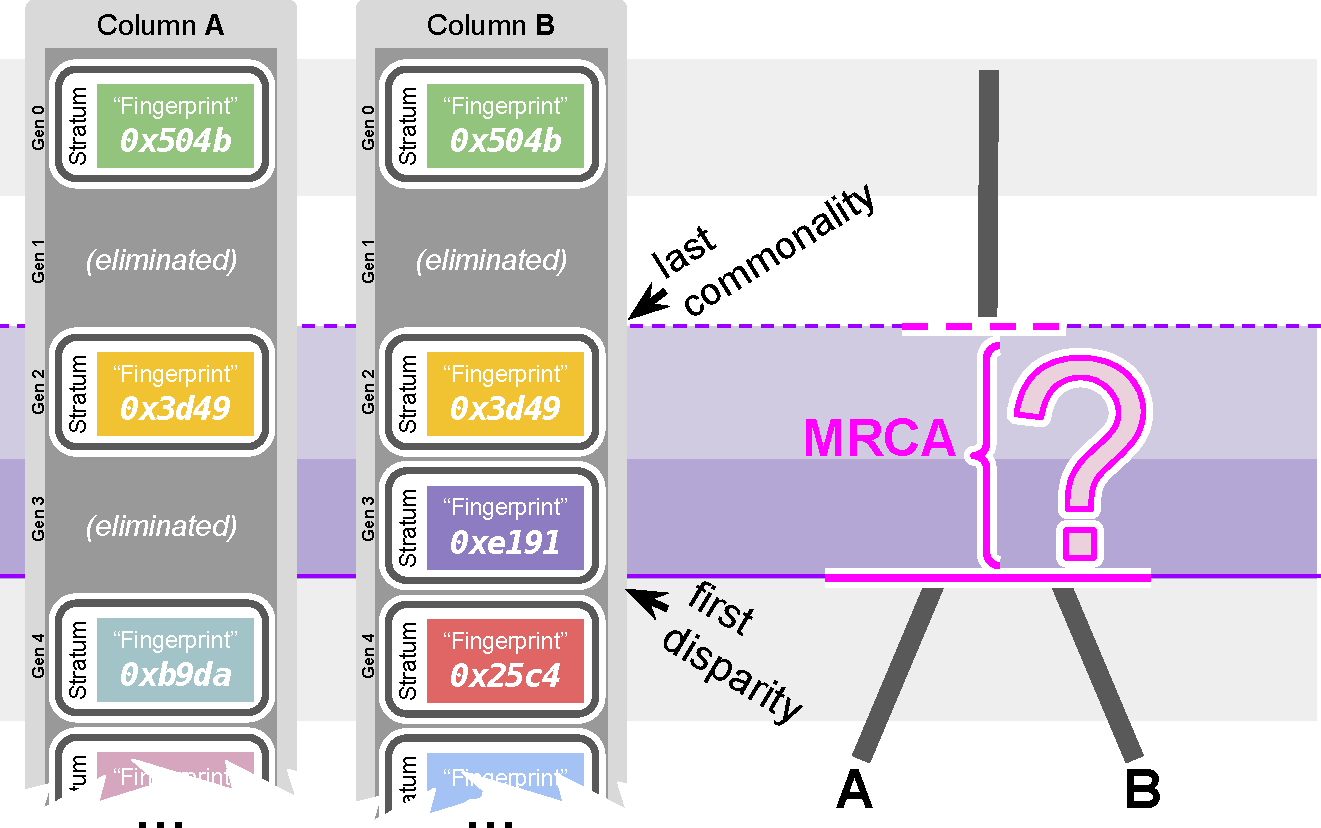
\includegraphics[width=\columnwidth]{img/column-comparison}
    \caption{
    Inferring the generation of the most-recent common ancestor (MRCA) of two hereditary stratigraphic columns $A$ and $B$.
    Columns are aligned at corresponding generations then the first generation with disparate ``fingerprints'' is determined.
    % (If a particular generation's strata have been eliminated from one or both columns or have not yet been deposited on one column, then no comparison is performed at that generation.)
    This provides a hard upper bound on the generation of the MRCA: these strata \textit{must} have been deposited along separate lines of descent.
    Then, searching backward for first commonality preceding that disparity provides a soft lower bound on the generation of the MRCA: these strata evidence common ancestry but \textit{might} collide by chance.
    % (If a narrow ``fingerprint'' differentia like a single bit is used with plausible collision probability, a lower bound can be established by continuing to search backward until the probability of $k$ successive spurious collisions is sufficiently unlikely.)
    % This process yields certainty about the phylogenetic relationship between $A$ and $B$ shown at right above (i.e., common) and below (i.e., diverged) the MRCA bounds.
    }
  \label{fig:column-comparison}
\end{figure}


Our algorithm, particularly the vocabulary we developed to describe it, draws on the concept of geological stratigraphy, inference of natural history through analysis of successive layers of geological material \citep{steno1916prodromus}.
As an introductory intuition, suppose a body of rock being built up through regular, discrete events depositing of geological material.
Note that in such a scenario we could easily infer the age of the body of rock by counting up the number of layers present.
% Note that it is crucial to this scenario that each layer has some differentiating feature that allows it to be distinguished from layers above and below it, but also potentially from layers present in another body of rock in a distant and unrelated geographic position.
Next, imagine making a copy of the rock body in its partially-formed state and then moving it far away.
As time runs forward on these two rock bodies, independent layering processes will cause consistent disparity in the layers forming on each forwards from their point of separation.

To deduce the historical relationship of these rock bodies after the fact, we could simply align and compare their layers.
Layers from their base up through the first disparity would correspond to shared ancestry; further disparate layers would correspond to diverged ancestry.
% Interestingly, and powerfully for phylogenetic inference, we can readily distinguish a scenario where both rock bodies deposited ten layers after diverging from a scenario where one deposited eighteen layers and the other deposited two.
Figure \ref{fig:column-comparison} depicts the process of comparing columns for phylogenetic inference.

Shifting now from intuition to implementation, a fixed-length randomly-generated binary tag provides a convenient and efficient mechanism to differentiate between our metaphorical ``layers.''
We call this ``fingerprint'' tag a \textit{differentia}.
The width of this tag controls the probability of spurious collisions between independently generated instances.
At 64 bits wide the tag essentially functions as a UID: collisions between randomly generated tags are so unlikely ($p < 5.42\times10^{-20}$) they can essentially be ignored.
At the other end of the spectrum, collision probability would be $1/256$ for a single byte and $1/2$ for a single bit.
In the case of narrow differentia, in order to set a lower bound for the MRCA generation, you would have to backtrack common strata from the last commonality until the probability of that many successive spurious collisions was enough to satisfy your desired confidence level (e.g., 95\% confidence).
Even then, there would be a possibility of the the true MRCA falling before the lower bound.
Note, however, that no matter the width of the differentia the generation of the first discrepancy provides a hard upper bound on the generation of the MRCA.

In accordance with our geological analogy, we refer to the packet of data accumulated each generation as a \textit{stratum}.
This packet contains the differentia and, although not employed in this work, could hold other arbitrary user-defined data (i.e., simulation timestamp, phenotype characteristics, etc.).
Again in accordance with the geological analogy, we refer to the chronological stack of strata that accumulate over successive depositions as a \textit{hereditary stratigraphic column}.

\subsection{Stratum Retention Policy}

\begin{figure*}
  \begin{minipage}{0.6\textwidth}
    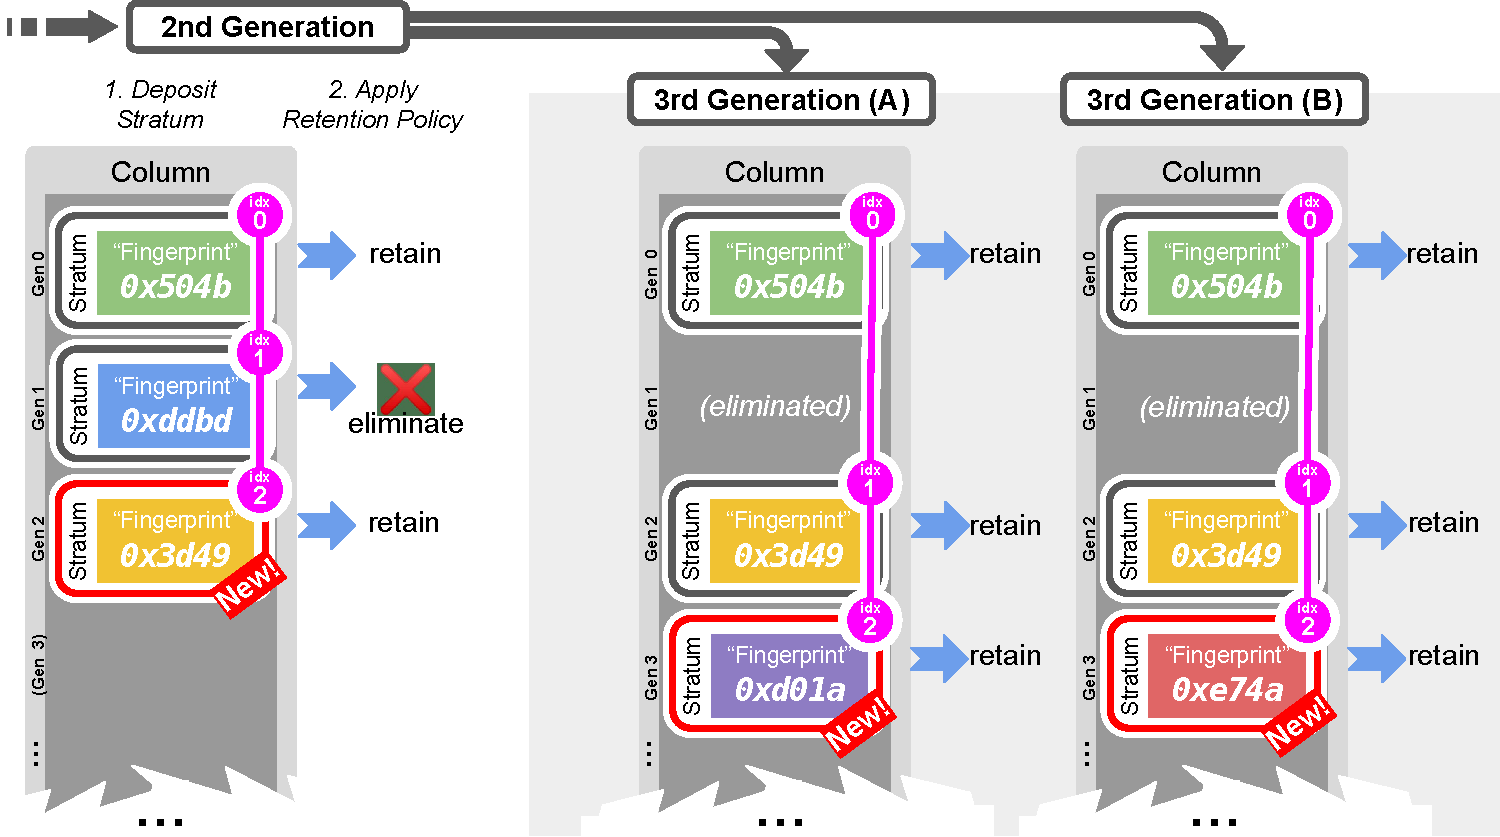
\includegraphics[width=\textwidth]{img/deposit-process}
  \end{minipage}%
  \begin{minipage}{0.4\textwidth}
    \caption{
    Cartoon illustration of stratum deposit process.
    This process marks the elapse of a generation when a hereditary stratigraphic column is inherited by an offspring.
    First, a new stratum is appended to the end of the column with a randomly-generated ``fingerprint.''
    This ``fingerprint'' distinguishes strata that were generated along disparate lines of descent (e.g., \texttt{0xd01a} for 3rd Generation A and \texttt{0xe74a} for 3rd generation B).
    Then, the column's configured stratum retention policy is applied to ``prune'' the column by eliminating strata from specific generations.
    Although this cartoon depicts an empty space for eliminated strata, the underlying data structure behind a column (i.e., the pink overlay) can condense to reduce space complexity.
    }\label{fig:deposit-process}
  \end{minipage}
\end{figure*}


As currently stated, fingerprints will accumulate proportionally to the length of evolutionary history simulated.
In an evolutionary run with thousands or millions of generations, this approach would soon become intractable --- particularly when columns are serialized and transmitted between distributed computing elements.
To solve this problem, we can trade off precision for compactness by deleting strata from columns as time progresses.
Figure \ref{fig:deposit-process} overviews how stratum deposit and stratum elimination progress over two generations under the hereditary stratigraphic column scheme.

Different patterns of deletion will lead to different trade-offs, both in terms of the scaling relationship of column size to generations elapsed and in terms of the arrangement of precision over evolutionary history (i.e., focusing precision on more recent evolutionary history versus spreading it evenly over the entire history).

We refer to the rule set used to selectively eliminate strata over time as the ``stratum retention policy.''
We explore several different retention policy designs here, and implement our software to allows for free, modular interchange of retention policies.
It is possible to define a policy through either of two mechanisms.
First, policy can be defined as a ``predicate'' where the generation of a stratum and the current number of strata deposited is passed into a function that returns whether that strata should be retained at that point in time.
Second, policy can be defined as a ``condemner'' generator where, given the current number of strata deposited, the set of ranks that should be deleted at this point in time are yielded.
Although the predicate form is useful for analyzing and proving properties of policies, the condemner form is generally more efficient in practice.
We provide predicate and condemner implementations for each stratum retention policy discussed here.

It should be noted that condemners and predicates are both defined in terms of stratum generation, not stratum index among retained strata in the column.
Therefore, it may seem necessary to store the generation of deposit within the stratum data structure.
However, if you know the total number of generations deposited you can map backwards from index to recover the generation deposited without storing it.
We provide this formula for each stratum retention policy.
Finally, for each policy we provide a formula to calculate the exact number of strata retained under any parameterization after $n$ generations.

In the next subsections, we introduce several stratum retention policies, provide the intuition behind their implementation, and elaborate their space complexity and resolution properties.
For each policy, patterns of stratum retention are illustrated in Figure \ref{fig:retention-policies}.
The formulas for number of strata retained after $n$ generations, the formulas to calculate stratum deposit generation from column index, and the retention predicate specifications of each policy are available in Supplementary Listing \ref{lst:StratumRetentionPredicateDepthProportionalResolution} \citep{moreno2022hstratconceptsupplement}.
The condemner generator specification of each policy is available in Supplementary Listing \ref{lst:StratumRetentionCondemnerDepthProportionalResolution} \citep{moreno2022hstratconceptsupplement}.
For tapered depth-proportional resolution and recency-proportional resolution, the accuracy of MRCA estimation can also be explored via an interactive in-browser web applet at \url{https://hopth.ru/bi}.

% \pragmaonce

% adapted from https://www.overleaf.com/learn/latex/Commands
\providecommand{\dissertationelse}[2]{%
% adapted from https://tex.stackexchange.com/a/33577
\ifdefined\DISSERTATION
#1
\else
#2
\fi
}

../../tex/lib/dissertationonly.tex

\begin{figure*}
  \centering
  \dissertationonly{\footnotesize}
  \begin{tabular}{m{0.05\textwidth}@{}|c@{}|c@{\hskip 0.01\textwidth}|m{0.14\textwidth}}
%-------------------------------------------------------------------------------
\hspace{-1ex}Policy&Lower-Resolution Parameterization&Higher-Resolution Parameterization&\makecell[c]{Properties}\\\hline
%-------------------------------------------------------------------------------
    \rotatebox{90}{\textbf{Fixed Resolution}}
  &
    \makecell{
      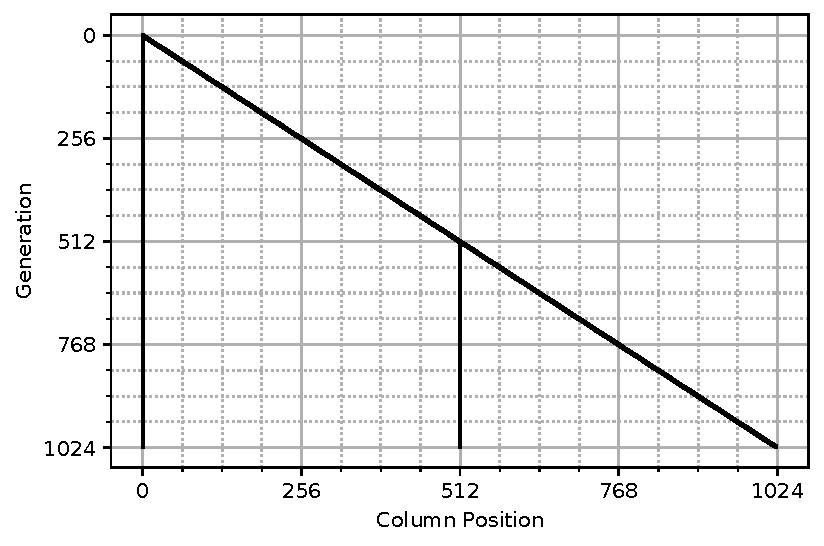
\includegraphics[valign=t,width=\dissertationelse{0.3}{0.4}\textwidth]{submodules/hereditary-stratigraph-concept/binder/retention-policies/teeplots/fixed_resolution=512+num_layers=1024+stratum_retention_predicate=fixed-resolution+viz=tweaked-stratum-retention-drip-plot+ext=}
    }
  &
    \makecell{
      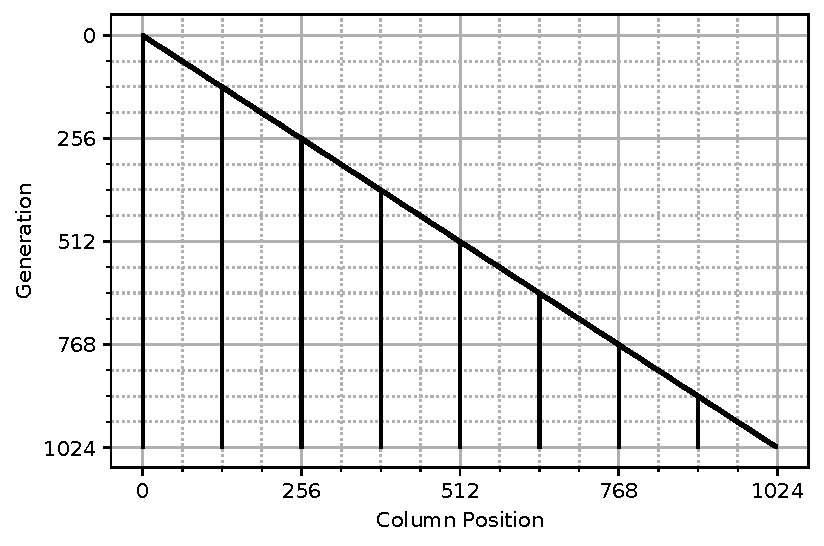
\includegraphics[valign=t,width=\dissertationelse{0.3}{0.4}\textwidth]{submodules/hereditary-stratigraph-concept/binder/retention-policies/teeplots/fixed_resolution=128+num_layers=1024+stratum_retention_predicate=fixed-resolution+viz=tweaked-stratum-retention-drip-plot+ext=}
    }
  &
  \makecell[{{p{0.14\textwidth}}}]{
  \centering
    \bf{Space Complexity}\\
    $O(n)$\\
    \bf{MRCA Uncertainty}\\
    $O(1)$
  }
  \makecell[{{p{0.14\textwidth}}}]{
  \raggedright
    where $n$ is gens elapsed.
  }\\\hline
%-------------------------------------------------------------------------------
    \adjustbox{
      minipage=10em,
      rotate=90,
    }{
      \centering
      \textbf{Depth-Proportional Resolution}
      \par
    }
  &
    \makecell{
      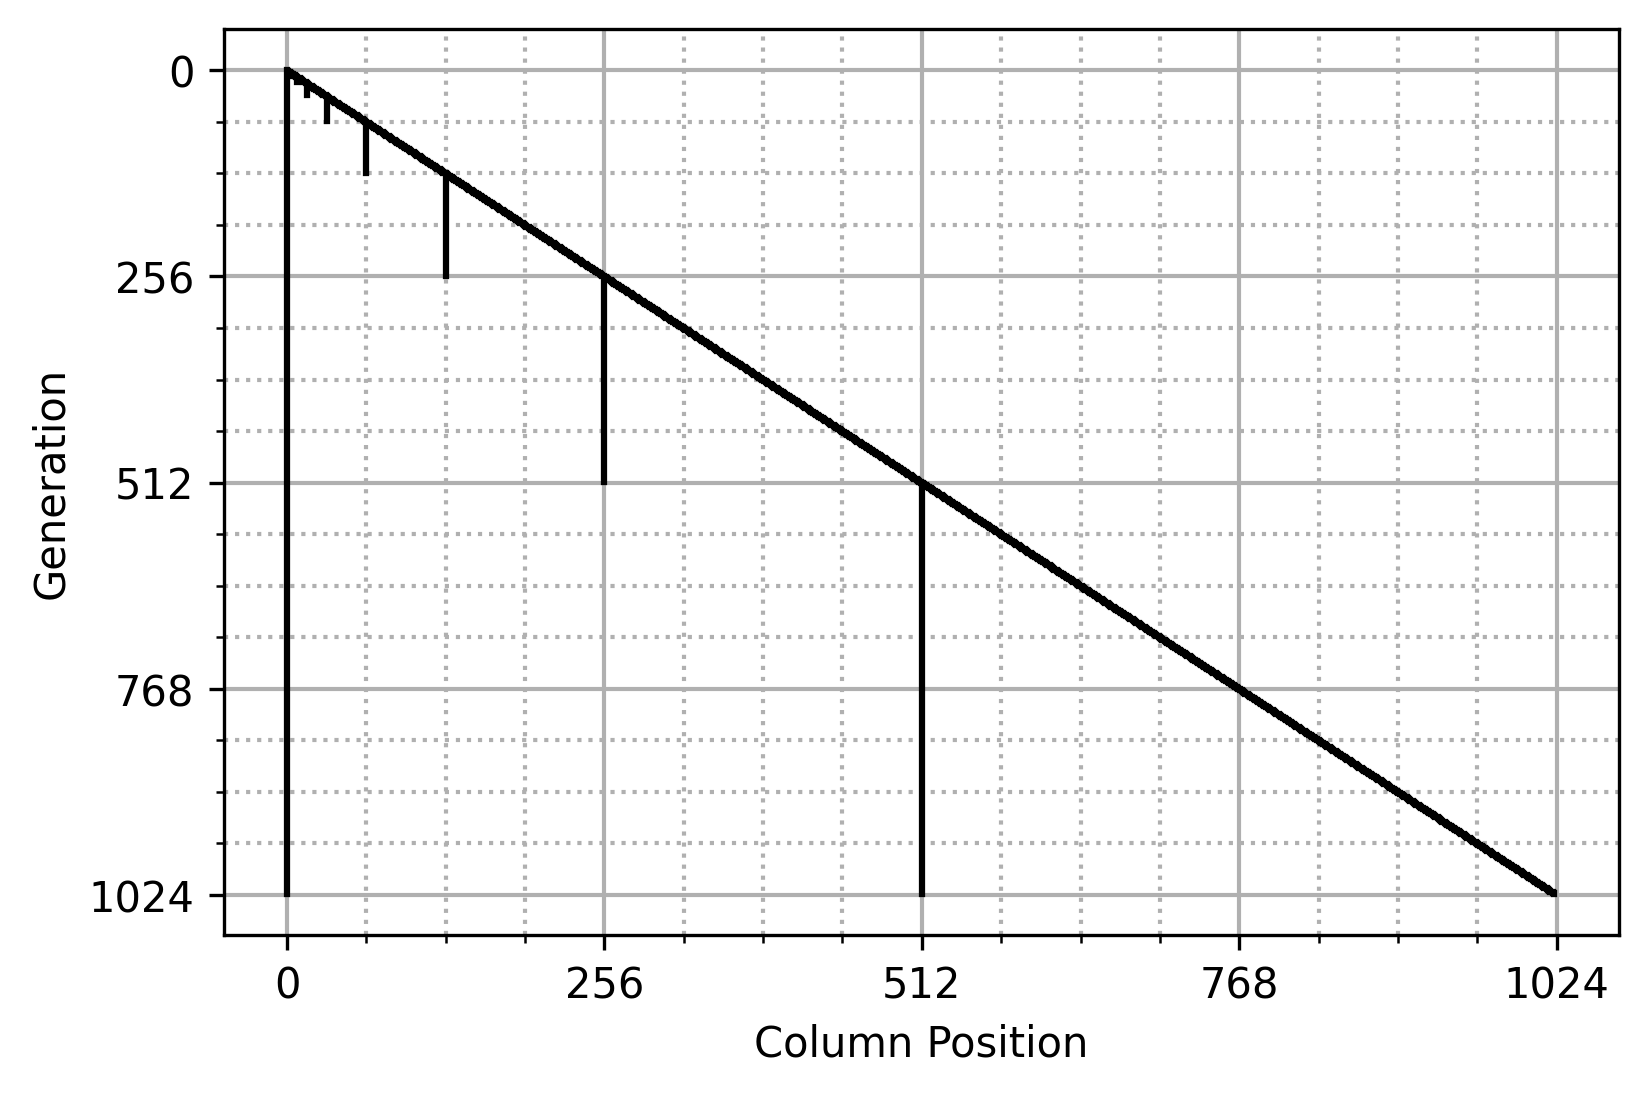
\includegraphics[valign=t,width=\dissertationelse{0.3}{0.4}\textwidth]{submodules/hereditary-stratigraph-concept/binder/retention-policies/teeplots/guaranteed_depth_proportional_resolution=1+num_layers=1024+stratum_retention_predicate=depth-proportional-resolution+viz=tweaked-stratum-retention-drip-plot+ext=}
    }
  &
    \makecell{
      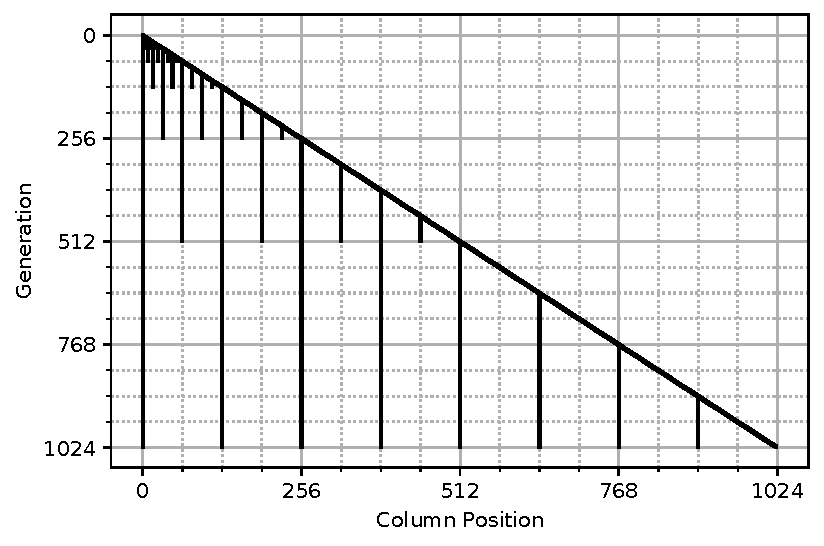
\includegraphics[valign=t,width=\dissertationelse{0.3}{0.4}\textwidth]{submodules/hereditary-stratigraph-concept/binder/retention-policies/teeplots/guaranteed_depth_proportional_resolution=4+num_layers=1024+stratum_retention_predicate=depth-proportional-resolution+viz=tweaked-stratum-retention-drip-plot+ext=}
    }
  &
  \makecell[{{p{0.14\textwidth}}}]{
  \centering
    \bf{Space Complexity}\\
    $O(1)$\\
    \bf{MRCA Uncertainty}\\
    $O(n)$
  }
  \makecell[{{p{0.14\textwidth}}}]{
  \raggedright
    where $n$ is gens elapsed.
  }\\\hline
%-------------------------------------------------------------------------------
    \adjustbox{
      minipage=15em,
      rotate=90,
    }{
      \centering
      \textbf{Tapered Depth-Proportional Resolution}
      \par
    }
  &
    \makecell{
      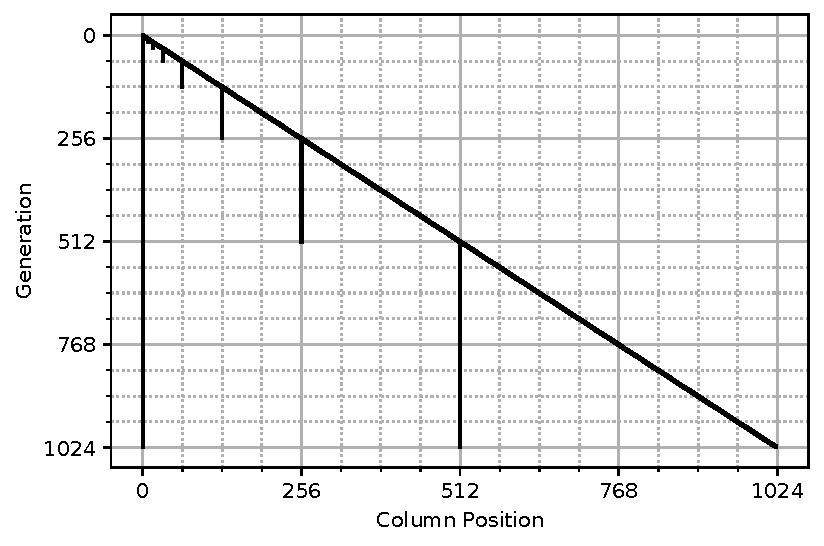
\includegraphics[valign=t,width=\dissertationelse{0.3}{0.4}\textwidth]{submodules/hereditary-stratigraph-concept/binder/retention-policies/teeplots/guaranteed_depth_proportional_resolution=1+num_layers=1024+stratum_retention_predicate=tapered-depth-proportional-resolution+viz=tweaked-stratum-retention-drip-plot+ext=}
    }
  &
    \makecell{
      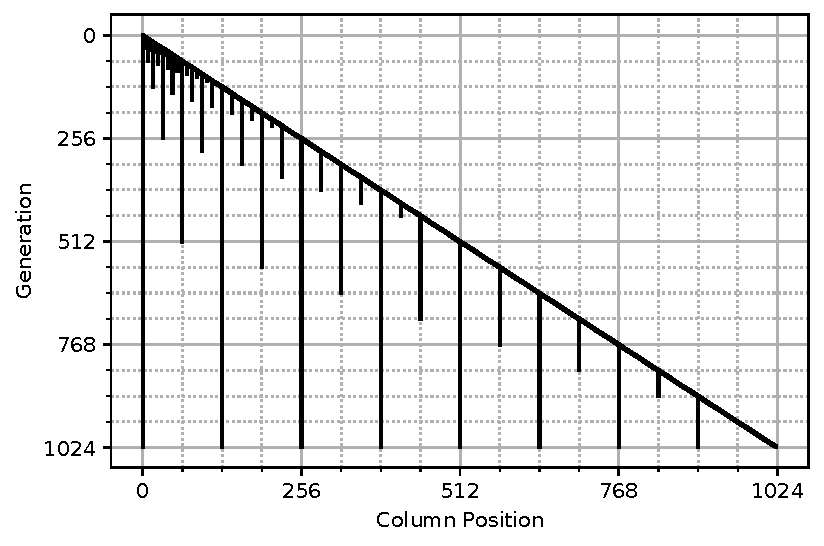
\includegraphics[valign=t,width=\dissertationelse{0.3}{0.4}\textwidth]{submodules/hereditary-stratigraph-concept/binder/retention-policies/teeplots/guaranteed_depth_proportional_resolution=4+num_layers=1024+stratum_retention_predicate=tapered-depth-proportional-resolution+viz=tweaked-stratum-retention-drip-plot+ext=}
    }
  &
  \makecell[{{p{0.14\textwidth}}}]{
  \centering
    \bf{Space Complexity}\\
    $O(1)$\\
    \bf{MRCA Uncertainty}\\
    $O(n)$
  }
  \makecell[{{p{0.14\textwidth}}}]{
  \raggedright
    where $n$ is gens elapsed.
  }\\\hline
%-------------------------------------------------------------------------------
  \adjustbox{
    minipage=15em,
    rotate=90,
  }{
    \centering
    \textbf{Recency-Proportional\\Resolution}
    \par
  }
  &
  \makecell{
    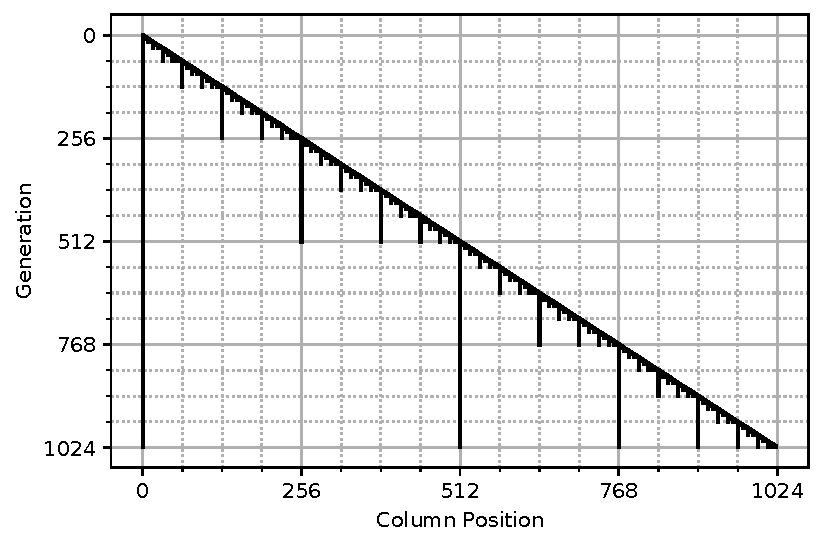
\includegraphics[valign=t,width=\dissertationelse{0.3}{0.4}\textwidth]{submodules/hereditary-stratigraph-concept/binder/retention-policies/teeplots/guaranteed_mrca_recency_proportional_resolution=0+num_layers=1024+stratum_retention_predicate=recency-proportional-resolution+viz=tweaked-stratum-retention-drip-plot+ext=}
  }
  &
  \makecell{
    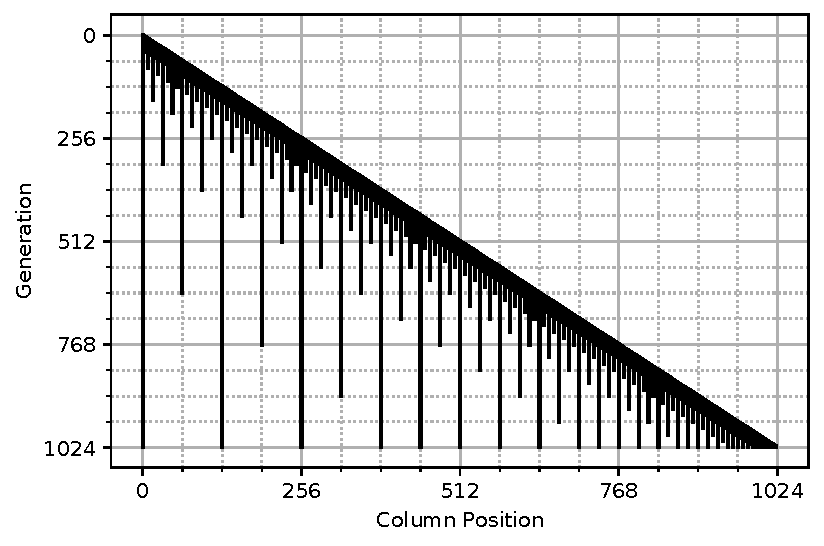
\includegraphics[valign=t,width=\dissertationelse{0.3}{0.4}\textwidth]{submodules/hereditary-stratigraph-concept/binder/retention-policies/teeplots/guaranteed_mrca_recency_proportional_resolution=4+num_layers=1024+stratum_retention_predicate=recency-proportional-resolution+viz=tweaked-stratum-retention-drip-plot+ext=}
  }
  &
  \makecell[{{p{0.14\textwidth}}}]{
  \centering
  \bf{Space Complexity}\\
  $O(\log(n))$\\
  \bf{MRCA Uncertainty}\\
  $O(m)$
  }
  \makecell[{{p{0.14\textwidth}}}]{
  \raggedright
  where $m$ is gens since MRCA and $n$ is total gens elapsed.
  }\\


  \end{tabular}
  \caption{
  Comparison of stratum retention policies.
  Policy visualizations show retained strata in black.
  Time progresses along the $y$-axis from top to bottom.
  New strata are introduced along the diagonal and then ``drip'' downward as a vertical line until eliminated.
  The set of retained strata present within a column at a particular generation $g$ can be read as intersections of retained vertical lines with a horizontal line with intercept $g$.
  Policy visualizations are provided for two parameterizations for each policy: the first where the maximum uncertainty of MRCA generation estimates would be 512 generations and the second where the maximum uncertainty of MRCA generation estimates would be 128 generations.
  }
  \label{fig:retention-policies}
\end{figure*}


\subsection{Fixed Resolution Stratum Retention Policy}

The fixed resolution retention policy provides a fixed absolute upper bound $r$ on the spacing between retained strata.
The strategy to obtain this property is simple: permanently retain a stratum every $r$th generation
(although, for arbitrary reasons of implementation convenience we require each stratum to be retained during at least the generation it is deposited).

However, this retention policy suffers from linear growth in a column's memory footprint with respect to number of generations elapsed: every $r$th generation generation a new stratum is permanently retained
For this reason, it is likely not useful in practice except potentially in scenarios where the number of generations is fixed in advance.
We include it here largely for illustrative purposes as a gentle introduction to retention policies.

\subsection{Depth-Proportional Resolution Stratum Retention Policy}

The depth-proportional resolution policy ensures spacing between retained strata will be less than or equal to a proportion $r$ of total number of strata deposited.
Achieving this limit on uncertainty requires retaining sufficient strata so that no more than $r$ ranks elapsed between any two strata.
This policy accumulates retained strata at a fixed interval until twice as many as $r$ are at hand.
Then, every other retained stratum is purged and the cycle repeats with a new twice-as-wide interval between retained strata.

When comparing stratigraphic columns from different generations, the resolution guarantee holds in terms of the number of generations experienced by the older of the two columns.
Because this retention policy is deterministic, for two columns with the same policy, every stratum that is held by the older column is also guaranteed to be present in the younger column (unless it hasn't yet been deposited on the younger column).
Therefore, the strata that would enable the desired resolution when comparing two columns of the same age are guaranteed to be available.

Because the number of strata retained under this policy is bounded as $2n+1$, space complexity scales as $O(1)$ with respect to the number of strata deposited.
It follows that the MRCA rank estimate uncertainty scales as $O(n)$ with respect to the number of strata deposited.

\subsection{Tapered Depth-Proportional Resolution Stratum Retention Policy}

This policy refines the depth-proportional resolution policy to provide a more stable column memory footprint over time.
The naive depth-proportional resolution policy builds up strata until twice as many are present as needed then purges half of them all at once.
The tapered depth-proportional resolution policy functions identically to the depth-proportional policy except that it removes unnecessary strata gradually from back to front as new strata are deposited, instead of eliminating them simultaneously.
The column footprint stability of this variation makes it easier to parameterize our experiments to ensure comparable end-state column footprints for fair comparison between retention policies, in addition to making this policy likely better suited to most use cases.
By design, this policy has the same space complexity and MRCA estimation uncertainty scaling relationships with number generations elapsed as the naive depth-proporitonal resolution policy.

\subsection{MRCA-Recency-Proportional Resolution Stratum Retention Policy}

\begin{table}
{\footnotesize
\begin{tabularx}{\columnwidth}{c | X | X | X | X}%
  \multirow{2}{*}{\makecell{\bfseries Num\\ \bfseries Generations \\ \bfseries Elapsed}}& \multicolumn{4}{m{0.6\columnwidth}}{\bfseries \centering
  Guaranteed MRCA-Recency-Proportional Resolution}\\ % specify table head
  \bfseries  & 1 & 4 & 10 & 100\\\hline\hline  % specify table head
  \csvreader[
    filter expr={
          test{\ifnumgreater{\thecsvinputline}{2}}
    }
  ]{submodules/hereditary-stratigraph-concept/binder/retention-policies/a=space-complexity+policy=recency-proportional-resolution+ext=.csv}{}% use head of csv as column names
{\num[scientific-notation=true,round-precision=2,round-mode=figures]{\csvcolii} & \csvcoliii & \csvcoliv & \csvcolv & \csvcolvi\\}% specify your columns here
\end{tabularx}
}
\caption{
Number strata retained after one thousand, one million, one billion, and one trillion generations under the recency-proportional resolution stratum retention policy.
Four different policy parameterizations are shown, the first where MRCA generation can be determined between two extant columns with a guaranteed relative error of 100\%, the second 25\%, the third 10\%, and the fourth 1\%.
A column's memory footprint will be a constant factor of these retained counts based on the fingerprint differentia width chosen.
For example, if single byte differentia were used, the column's memory footprint in bits would be $8\times$ the number of strata retained.
} \label{tab:recency-proportional-space-complexity}
\end{table}


The MRCA-recency-proportional resolution policy ensures distance between the retained strata surrounding any generation point will be less than or equal to a user-specified proportion $r$ of the number of generations elapsed since.

This policy can be constructed recursively, so to begin, let's consider setting up just the \textit{first} generation $g$ of the stratum after the root ancestor we will retain when $n$ generations have elapsed.
A simple geometric analysis reveals that providing the guaranteed resolution for the worst-case generation within the window between generation 0 and generation $g$ (i.e., generation $g-1$) requires
\begin{align*}
  g \leq \lfloor n / (r + 1) \rfloor.
\end{align*}

We now have an upper bound for the rank of the first stratum generation we must retain.
However, we must guarantee that these ranks are actually available for us to retain (i.e., it hasn't been purged out of the column at a previous time point as the column was grown by successive deposition).
We will do this by picking the rank that is the highest power of 2 less than or equal to our bound.
If we repeat this procedure as we recurse, we are guaranteed that this rank will have been preserved across all previous timepoints.

Why does this work?
Consider a sequence where all elements are powers of 2 and elements in the sequence are strictly nonincreasing.
Consider the first element of the list.
Partial sums along the sequence will include all multiples this first element.
So, when we ratchet up $g$ to $2g$ as $n$ increases, we are guaranteed that $2g$ has been retained.
This principle generalizes recursively down the list.
This is a similar principle to the approach of strictly-doubling interval sizes used in the Naive and Tapered Depth-Proportional Resolution stratum retention policies described above.

This step of truncating to the nearest less than or equal to power of 2 affects our recursive step size at most only by a constant factor of 2.
So, because step size is a constant fraction of remaining generations $n$ (at worst $\frac{1}{2(r+1)}$), the number of steps made (and number of strata retained) scales as $O(\log(n))$ with respect to the number of strata deposited.
Table \ref{tab:recency-proportional-space-complexity} provides exact figures for the number of strata retained under different parameterizations of the recency-proportional retention policy between one thousand and one trillion generations.

As for rank estimate uncertainty, in the worst case it scales as $O(n)$ with respect to the greater number of strata deposited.
However, with respect to estimating the rank of the MRCA when lineages diverged any fixed number of generations ago, uncertainty scales as $O(1)$.

How does space complexity scale with respect to the policy's specified resolution $r$?
Through extrapolation from OEIS sequences A063787 and A056791 via guess and check \citep{sloane2021a063787,sloane2021a056791}, we posited the exact number of strata retained after $n$ generations as

\begin{align*}
  \mathrm{HammingWeight}(n)
  + \sum_1^r \lfloor \log_2( \lfloor n / r \rfloor ) \rfloor
  + 1.
\end{align*}

This expression has been unit tested extensively to ensure perfect reliability.
Approximating and applying logarithmic properties, this policy's space complexity can be calculated within a constant factor as

\begin{align*}
\log(n) + \log\Big(\frac{n^r}{r!}\Big).
\end{align*}

To answer our question, we will examine the ratio of space complexities required when scaling resolution $r$ up by a constant factor $f > 1$.
Evaluating this ratio as $r \to \infty$, we find that space complexity scales directly proportional with the desired resolution $r$ at the limit,

\begin{align*}
\lim_{r \to \infty}
\frac{
  \log(n) + \log\Big(\frac{n^{fr}}{(fr)!}\Big)
}{
  \log(n) + \log\Big(\frac{n^r}{r!}\Big)
}
= f.
\end{align*}

Evaluating this ratio as $n \to \infty$, we find that this scaling relationship is never worse than directly proportional for any $r$,

\begin{align*}
\lim_{n \to \infty}
\frac{
  \log(n) + \log\Big(\frac{n^{fr}}{(fr)!}\Big)
}{
  \log(n) + \log\Big(\frac{n^r}{r!}\Big)
}
&= \frac{fr+1}{r+1}\\
&= f\frac{r + 1/f}{r + 1}\\
&\leq f.
\end{align*}


\subsection{Computational Experiments}

In order to assess the practical performance of the hereditary stratigraph approach in an applied setting, we simulated the process of stratigraph propagation over known ``ground truth'' phylogenies extracted from pre-existing digital evolution simulations \citep{hernandez2022phylogenetic}.
These simulations propagated populations of between 100 and 165 bitstrings between 500 and 5,000 synchronous generations under the NK fitness landscape model \citep{kauffman1989nk}.
In order to ensure coverage of a variety of phylogenetic conditions, we sampled a variety of selection schemes that impose profoundly different ecological regimens \citep{dolson2018ecological},
\begin{itemize}
  \item EcoEA Selection \citep{goings2012ecology},
  \item Lexicase Selection \citep{helmuth2014solving},
  \item Random Selection,
  \item Sharing Selection \citep{goldberg1987genetic}
  % \item Tournament Selection \citep{miller1995genetic}.
\end{itemize}

Supplementary Table \ref{tab:ground-truth-phylogenies} provides full details on the conditions each ground truth phylogeny was drawn from.
The phylogenies themselves are available in our data repository for this project.

For each ground truth phylogeny, we tested combinations of three configuration parameters:
\begin{itemize}
  \item target end-state memory footprints for extant columns (64, 512, and 4096 bits),
  \item differentia width (1, 8, and 64 bits), and
  \item stratum retention policy (tapered depth-proportional resolution and recency-proportional resolution).
\end{itemize}

Stratum retention policies were parameterized so that the maximum number of strata possible were present at the end of the experiment without exceeding the target memory footprint.
If the target memory footprint is exceeded by the sparsest possible parameterization of a retention policy, then that sparsest possible parameterization is used.
Supplementary Tables \cref{tab:experiment-column-sizes-nk-ecoea-selection,tab:experiment-column-sizes-nk-lexicase-selection,tab:experiment-column-sizes-nk-random-selection,tab:experiment-column-sizes-nk-sharing-selection,tab:experiment-column-sizes-nk-tournament-selection} provide the calculated paramaterizations and memory footprints of extant columns \citep{moreno2022hstratconceptsupplement}.

In order to assess the viability of phylogenetic inference using hereditary stratigraphic columns from extant organisms, we used the end-state stratigraphs to estimate a reconstruction of the actual ground truth phylogenetic histories.
The first step to reconstructing a phylogenetic tree for the history of an extant population at the end of an experiment is to construct a distance matrix by calculating all pairwise phylogenetic distances between extant columns.
We defined phylogenetic distance between two extant columns as the sum of each extant organism's generational distance back to the generation of their MRCA, estimated as the mean of the upper and lower 95\% confidence bounds.
Supplementary Figure \ref{fig:phylogenetic-inference} provides a cartoon summary of the process of calculating phylogenetic distance between two extant columns \citep{moreno2022hstratconceptsupplement}.

We then used the unweighted pair group method with arithmetic mean (UPGMA) reconstruction tool provided by the BioPython package to generate estimate phylogenetic trees \citep{cock2009biopython,sokal1958statistical}.
After generating the reconstructed tree topology, we performed a second pass to adjust branch lengths so that each tree node sat at the mean of its estimated 95\% confidence generation bounds.
%We found that the neighbor joining (NJ) approach occasionally yielded reconstructions with impossible ``negative generation'' branches \citep{saitou1987neighbor} after knowledge bounding the absolute generation of internal nodes (i.e., MRCA's between pairs of extant organisms) was applied, so we did not use it.

\subsection{Software and Data}

% A prototype of this approach has been implemented \url{https://github.com/mmore500/dishtiny/blob/incoming/include/dish2/genome/PhyloFingerprints.hpp} and preliminarily tested \url{https://github.com/mmore500/dishtiny/blob/incoming/tests/dish2/genome/PhyloFingerprints.cpp}.

As part of this work, we published the \texttt{hstrat} Python library with a stable public-facing API intended to enable incorporation in other projects with extensive documentation and unit testing on GitHub at \url{https://anonymous.4open.science/r/hstrat-115D/} and on PyPI.% at \url{https://pypi.org/project/hstrat/}. https://github.com/mmore500/hstrat
In the near future, we intend to complete and publish a corresponding C++ library.

Supporting software materials can be found on GitHub at \url{https://anonymous.4open.science/r/hereditary-stratigraph-concept-6BEC/}.%\url{https://github.com/mmore500/hereditary-stratigraph-concept}
Supporting computational notebooks are available for in-browser use via BinderHub at \url{ANONYMIZED FOR PEER REVIEW} \citep{ragan2018binder}. %https://mybinder.org/v2/gh/mmore500/hereditary-stratigraph-concept/HEAD?labpath=binder%2F
Our work benefited from many pieces of open source scientific software, including \citep{sukumaran2010dendropy,virtanen2020scipy,hunter2007matplotlib,virtanen2020scipy,waskom2021seaborn,bostock2011d3,meurer2017sympy,smith2020treedistdata,paradis2004ape,ushey2022reticulate,wickham2022dplyr}.
The ground truth phylogenies used in this work as well as supplementary figures, tables, and text are available via the Open Science Framework at
\url{https://osf.io/4sm72/?view\_only=69f37c6d184143b7855299c3323749ea} \citep{foster2017open,moreno2022hstratconceptsupplement}.
Phylogenetic data associated with this project is stored in the Alife Community Data Standards format \citep{lalejini2019data}.
